\documentclass{beamer} 
%\documentclass[handout]{beamer} 

% Michael Maier, 2014.
% CC-BY-SA 3.0 at

\usepackage[utf8]{inputenc}
\usepackage[ngerman]{babel}

\title{OpenStreetMap - Die freie Weltkarte} 
\author{Michael Maier \textless Michael.Maier@student.tugraz.at\textgreater} 
\date{9. April 2014} 

\usetheme{Antibes}

\hypersetup{colorlinks=true,urlcolor=blue,linkcolor=white}

%\usebackgroundtemplatei{
%
\includegraphics[width=\paperwidth,
%height=0.8\paperheight]{mag_map.png}
%}

\begin{document}

%\maketitle

\begin{frame} 


\begin{figure}
  \centering
  
\includegraphics[width=.5\textwidth]{mag_map.png}
\end{figure}

\begin{center}
\Huge{OpenStreetMap\\}
\end{center}

\begin{center}
\Large{\emph{Die freie Weltkarte nutzen}}
\end{center}

\end{frame}


\section{Einleitung}


\begin{frame}{Vorstellung}

  \begin{itemize}
    \item Michael Maier \textless \href{mailto:Michael.Maier@student.tugraz.at}{Michael.Maier@student.tugraz.at}\textgreater
    \item Student an der TU Graz (Telematik)
\vspace{0.3cm}
    \item Linux-User (Debian/grml) seit 2004
    \item Organisiere Grazer Linuxtage seit 2011 mit
    \item OpenStreetMap als Hobby seit Juli 2010
    \item Leite den Grazer OSM-Stammtisch seit Mai 2011
\vspace{0.3cm}
    \item Vorträge und Workshops zum Thema OSM seit 2012
    \item Freiberuflich OSM-Aufträge und Consulting
    \begin{itemize}
      \item OSM-username: \emph{\href{http://www.openstreetmap.org/user/species}{species}}
      \item Github-Account: \emph{\href{https://github.com/species}{species}}
      \item Twitter-Account: \emph{\href{https://twitter.com/osmgraz}{@osmgraz}}
    \end{itemize}
  \end{itemize}
\end{frame}


% Folien zu
% * kurze OSM-Vorstellung, Geschichtliches, Motivation
%  1. OSM-Vorstellung
  % was ist es
  % wer steckt dahinter?
% Geschichtliches
  % Gegründet ... steve
  % user-wachstum
% Motivation
  % gegründet, weil es keine freien Geodaten gab
  % Wunschtraum: eine DB weltweit

\begin{frame}{Was ist OpenStreetMap}

\begin{itemize}
  \item OpenStreetMap (OSM) ist eine freie Weltkarte nach dem Wiki-Prinzip "`Wikipedia der Karten"'
    \begin{itemize}
      \item \emph{Eigentlich eine Geo-Datenbank}
    \end{itemize}
\pause
  \item Entsteht aus der Arbeit von \textgreater 1,4\,M Hobbykartografen "`\emph{Mapper}"'

 \item Das komplette "`planet file"' ist ca. 427\,GB groß (xml) (Dienstag):
  \begin{itemize}
    \item 2.161.810.973 Nodes
    \item 213.302.643 Ways
    \item 2.326.786 Relations
  \end{itemize}

\end{itemize}


% \begin{center}
% 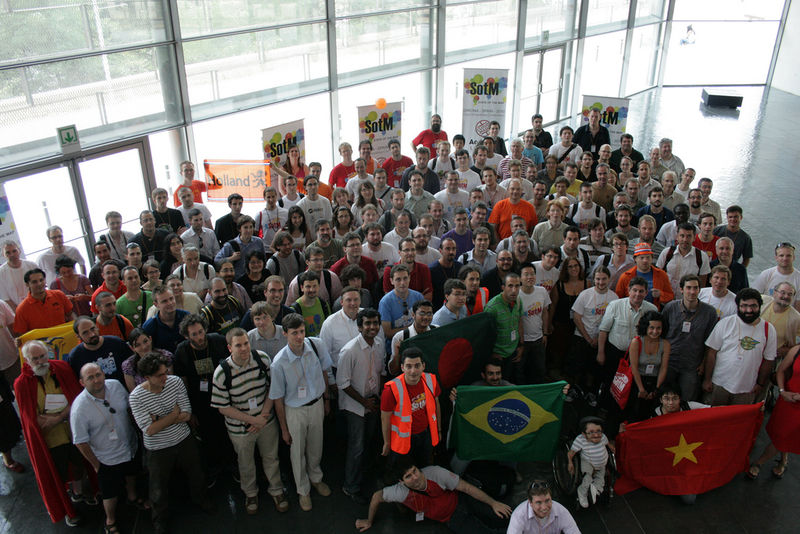
\includegraphics[width=5.5cm]{sotm.jpg}
% \end{center}

\end{frame}

\begin{frame}{Wer steht hinter OpenStreetMap}

  \begin{itemize}
    \item OpenStreetMap Foundation (Server, Rechtliche Vertretung)
      \pause
    \item Mapper ($\sim$20.000 aktiv), meist ohne Geo-Hintergrund
    \begin{itemize}
      \item Jährliche Konferenz - "`State of the Map"', heuer: Buenos Aires
    \end{itemize}
      \pause
    \item Universitäten
    \begin{itemize}
      \item Bakk-, Master- und Doktorarbeiten mit OSM
      \item Server-Hosting
    \end{itemize}
      \pause
    \item Organisationen, die Daten sponsern
    \begin{itemize}
      \item Firmen wie Yahoo/Bing, die Luftbilder zur Verfügung stellen
      \item Regierungen mit besseren Open-Data-Gesetzen als Österreich
  % BSP TIGER, USA
  % Dänemark, Hausnummern
  % Frankreich,Tschechien: Kataster
    \end{itemize}
      \pause
    \item Firmen die mit OSM arbeiten, z.B.:
    \begin{itemize}
      \item Geofabrik (de)
      \item MapQuest (us)
      \item BikeCityGuide (Graz)
    \end{itemize}
  \end{itemize}



\end{frame}

  
{
 \usebackgroundtemplate{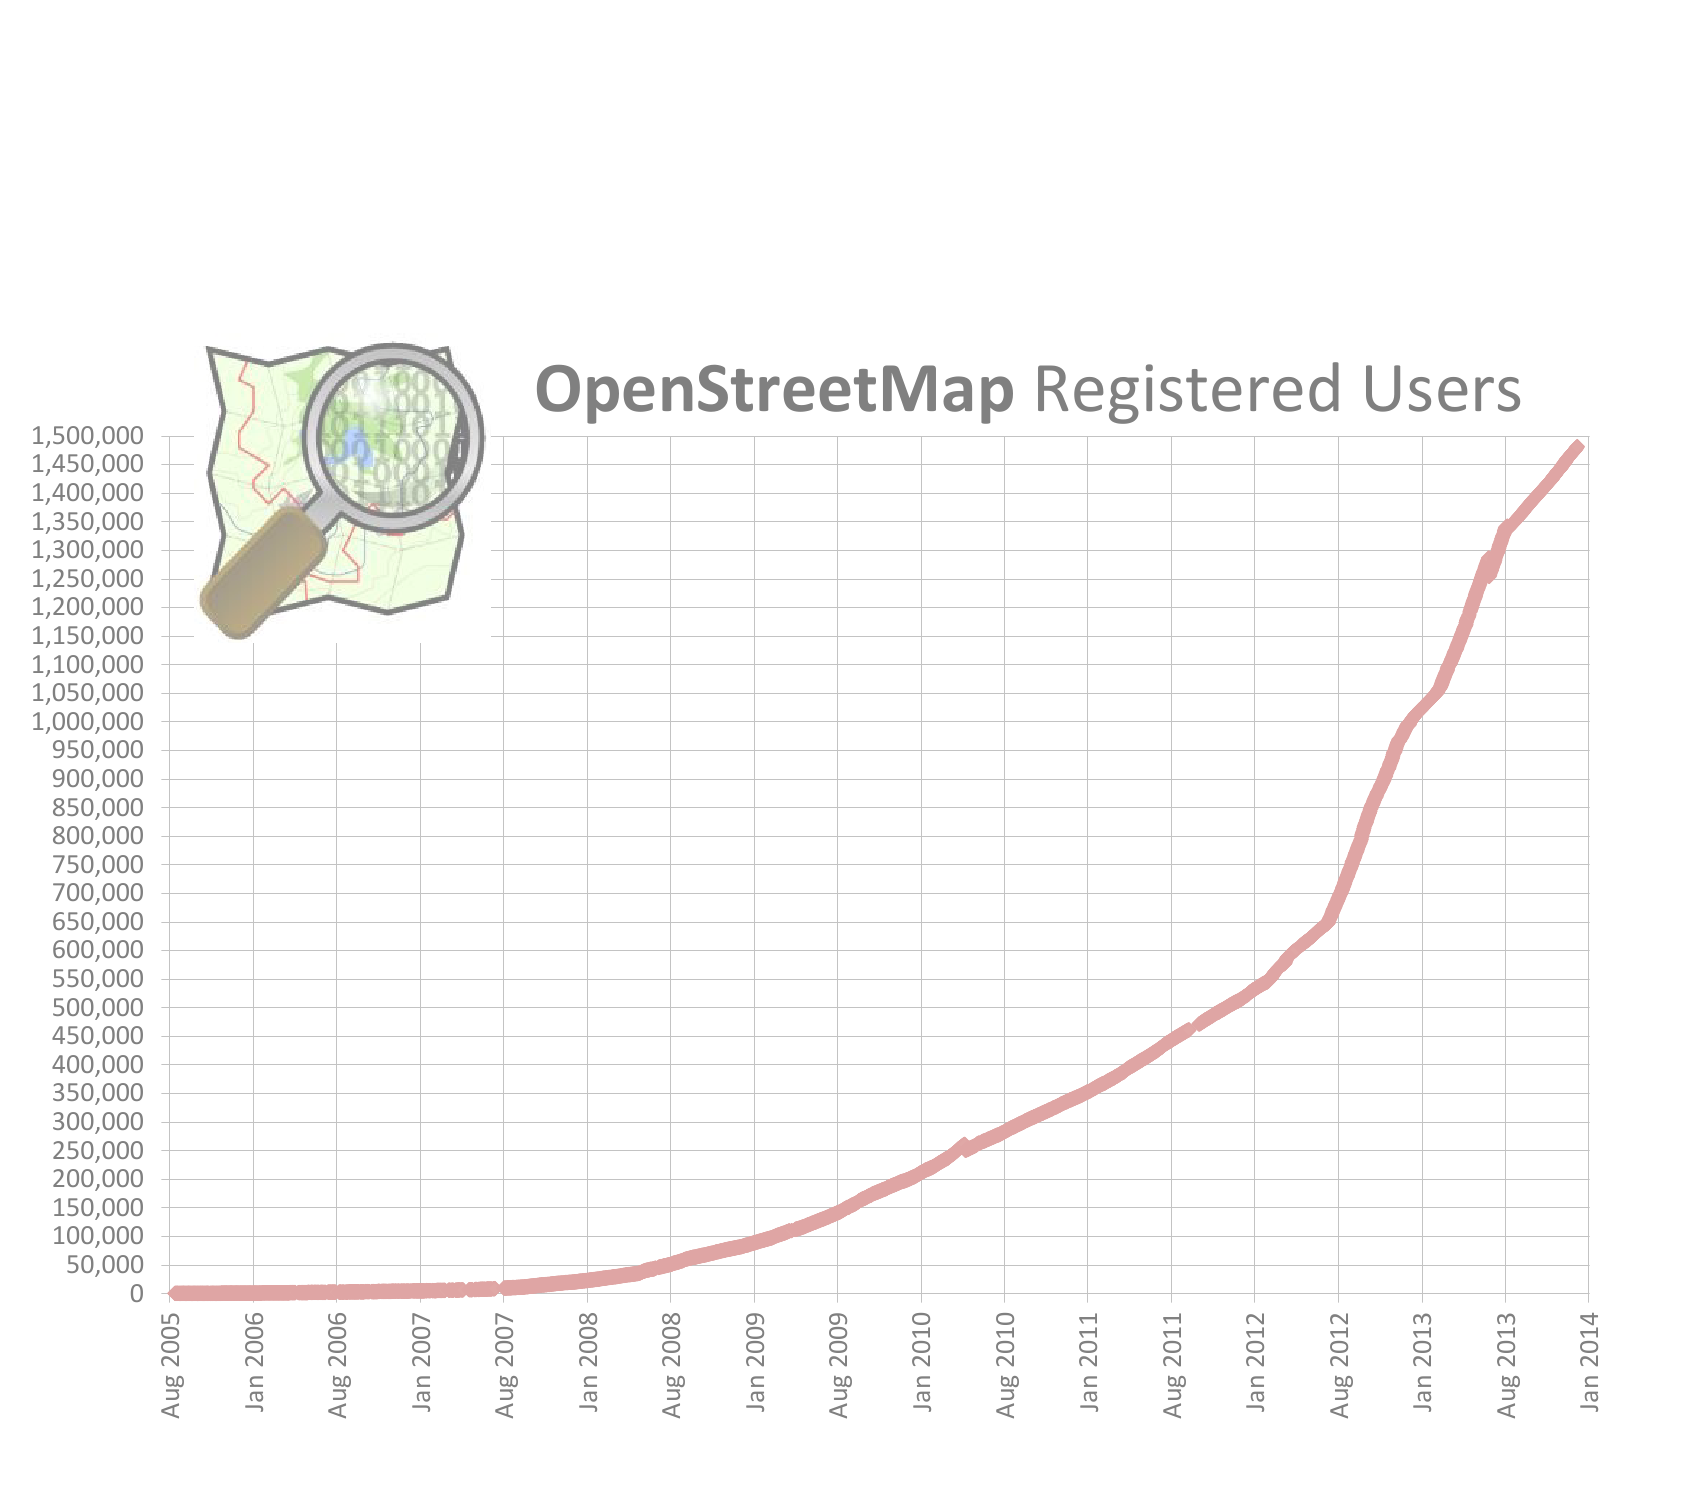
\includegraphics[height=10cm]{Osmdbstats2_users.png}}

\begin{frame}{Geschichte von OpenStreetMap}
  \vspace{0.6cm}
\begin{itemize}
  \item Start des Projekts im August 2004 durch \emph{Steve Coast}
  \item Dezember 2006 - Yahoo erlaubt abzeichnen
  \item Juli 2007 - Erste Konferenz, "`State Of The Map"'
  \item August 2007 - 10.000 Registrierte Benutzer
  \item März 2009 - 100.000 Registrierte Benutzer
  \item Januar 2010 - Haiti--Projekt
  \item November 2010 - Bing erlaubt abzeichnen
  \item Juli 2011 - Erste "`State Of The Map Europe"' in Wien
  \item Januar 2013 - 1.000.000 Registrierte Benutzer
  \item Gestern - 1.491.901 Registrierte Benutzer
\end{itemize}

\end{frame}
}




\begin{frame}{Warum OpenStreetMap?}

\hspace{0.5cm}Es beginnt 2004 mit einer Geschichte: 
  \vspace{0.3cm}

Ein Student ärgert sich, dass es in UK keine freien Geodaten gibt. 
  \vspace{0.3cm}

\parbox{9.5cm}{Die Daten auf streetmap.co.uk wurden mit Steuergeldern erstellt, man kann die Rohdaten jedoch nicht frei verwenden.}
\hfill
\raisebox{\dimexpr-\height+\baselineskip}{
\includegraphics[height=1cm]{traurig.png}}

  \vspace{0.6cm}
\pause

Warum muss man für etwas, was bereits von der Allgemeinheit mit Steuergeld bezahlt wurde, nocheinmal bezahlen?
  \vspace{0.3cm}

\parbox{9.1cm}{Und darf es selbst dann nicht frei Nutzen? \\Doppelbesteuerung ist zumindest bei uns verboten?}
\hfill 
\raisebox{\dimexpr-\height+\baselineskip}{
\includegraphics[height=1cm]{grantig.png}}

\pause

 \parbox{7.5cm}{\vspace{0.4cm}\hspace{0.5cm}$\Longrightarrow$ \hspace{0.5cm}Er gründet OpenStreetMap!} 
\raisebox{\dimexpr-\height+\baselineskip}{
\includegraphics[height=1.2cm]{laugh.png}}

\end{frame}

\begin{frame}{Vision einer besseren Geo-Welt}

 Sollte es nicht so sein:
  \begin{itemize}
    \item Es gibt weltweit EIN Portal für ALLE Geodaten 
    \item In einheitlichem Format (WGS84, Dezimalgrad und UTF-8)
    \item Alte Versionen verfügbar sind (Um Änderungen zu tracken)
    \item Unkompliziert Fehler melden, oder selbst ausbessern kann
\pause
    \item Man keine Anträge stellen muss, sondern einfach einen Ausschnitt wählt und Rohdaten runterlädt
    \item Alle Daten unter einen freien Lizenz nutzen kann
  \end{itemize}

  \begin{columns}[c]
        \column{.5\textwidth}
        \begin{center}
  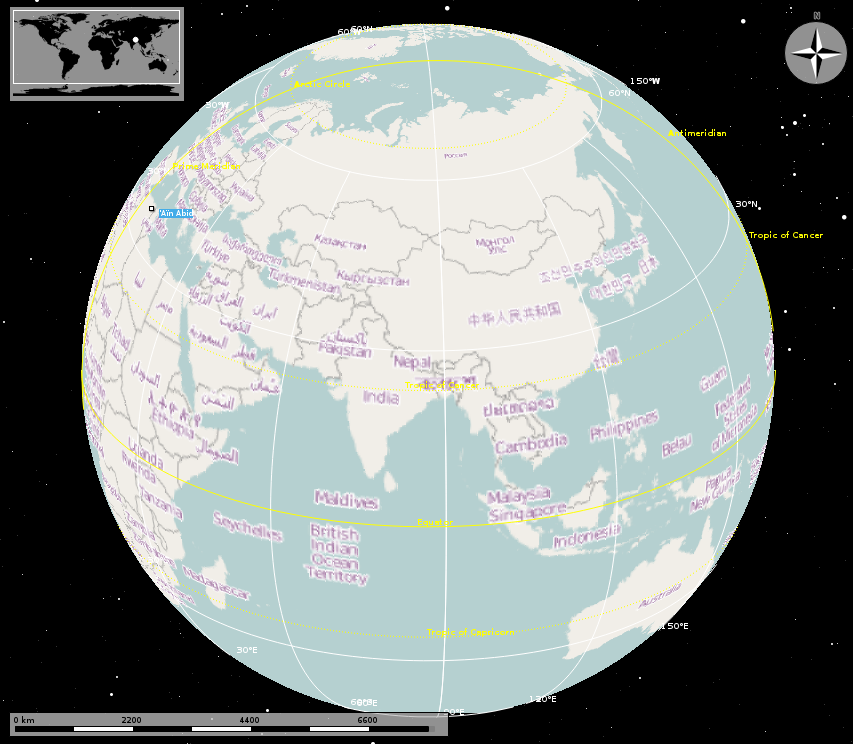
\includegraphics[width=3.5cm]{marble.png}
  \end{center}
        \column{.5\textwidth}
      \begin{center}
    
\includegraphics[width=2.5cm]{cc-by-sa.pdf}
  \end{center}
\end{columns}

\end{frame}


\begin{frame}{Humanitarian OSM Team}

\vspace{-1.5cm}
\hfill 
\includegraphics[width=5cm]{hot.png}

OSM ist nicht nur gemeinnützig, sondern es stehen auch tausende Mapper bereit, von zuhause aus im Katastrophenfall zu helfen.
\vspace{0.1cm}

Das HOT-Team unterstützt und arbeitet zusammen mit:

\begin{itemize}
  \item UN
  \item Weltbank
  \item Rotes Kreuz
\end{itemize}

Das erste Große Projekt: Haiti Januar 2010 (Erdbeben Stärke 7.0)

\begin{itemize}
  \item Es gab keine amtlichen Karten
  \item innerhalb von 48\,h waren hochauflösende Luftbilder der Nasa verfügbar
  \item  600 Mapper zeichneten "`from scratch"' die Karte, die vor Ort von den Hilfsorganisationen verwendet wurde
\end{itemize}

\end{frame}

\begin{frame}{HOT: Typhoon Haiyan 2013, Tasking manager}

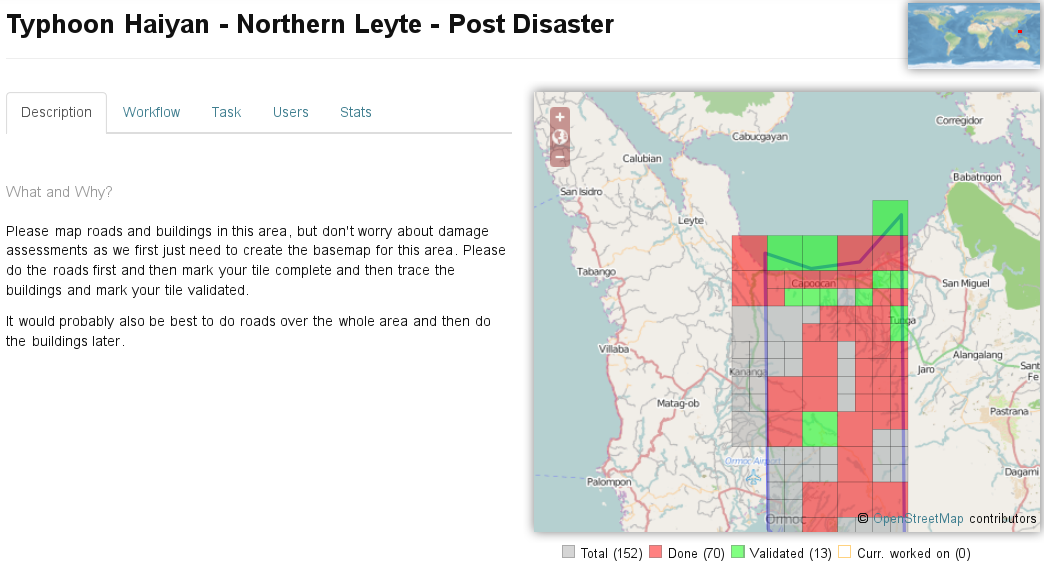
\includegraphics[width=10cm]{hot-task.png}

\begin{itemize}
  \item 1679 User erzeugen 4,8\,M Änderungen, neue Karten wurden vor Ort täglich zur Verfügung gestellt
  \item Mappen von Straßen, zerstörten Gebäuden und Infrastruktur
\end{itemize}

\end{frame}

\section{Wie funktioniert OpenStreetMap?}
% * Technogie, Datenmodell, Lizenz

\begin{frame}{Woher kommen unsere Daten?}

\begin{itemize}
  \item Ursprünglich: GPS-Tracks
  \item Freiwillige tragen ihr Wissen bei: Jeder weiß viel über seine Umgebung:
	\begin{itemize}
	  \item Hausnummern, Straßennamen,
	  \item Restaurants, Bars, POIs, \dots
  \end{itemize}
  \pause
  \item Bei Mapping-Parties werden \\ gezielt Gebiete verbessert
\end{itemize}

  \vspace{0.4cm}
 99\% Handarbeit!

  \vspace*{-2.9cm}
 \hfill 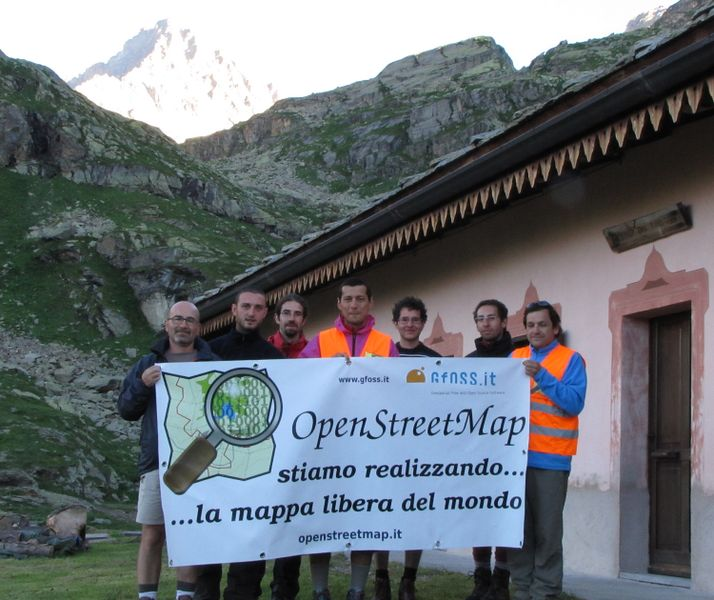
\includegraphics[width=4.2cm]{alps_mp.jpg}


  \pause
\begin{itemize}
  \item Hin und wieder Importe aus Open Government Data
  \begin{itemize}
    \item USA, TIGER Data (2008)
    \item Dänemark, Hausnummern (laufend synchronisiert)
    \item Wien, Baumkataster
  \end{itemize}
\end{itemize}

\end{frame}

\subsection{Technologie}

% 100% freie Software
% → jeder kann den Software-Stack verwenden http://openaviationmap.org/
% Quality Assurance
% * Es gibt automatische Q/A-Tools
% * kaum Streitfälle - wenn dann Mailinglist, Data Working Group
% * 
% tolle Bilder herzeigen!
% * irgendein Zoo
% * 3D -FIXME
% * Tolle Kartenstile:
%     * OSM-Fr?
%     * stamen watercolor
%     * pistemap
%     * bicycle map
%     * OpenSeaMap

\begin{frame}{Freie Software für freie Daten}

Nicht nur die Daten sind frei, sondern auch die Software um die Daten zu verwalten, generieren und verwenden.

\vspace{0.6cm}

Es wird zu 100\% Freie Software verwendet. Beispiel osm.org:
\begin{itemize}
  \item Hauptdatenbank: (PostgreSQL/PostGIS) 
  \item Renderstack: Mapnik/Tirex
  \item Webserver: Apache/mod\_tile
  \item Webfrontend: Leaflet
  \item Web-Backend: Basiert auf Ruby on Rails
  \item Doku-Portal: Mediawiki
\end{itemize}


  \vspace*{-3cm}
 \hfill 
\includegraphics[width=3cm]{tux.png}


\pause

Z.B verwendet \href{http://openaviationmap.org/}{openaviationmap.org} dieselben Technologien.

\end{frame}


\begin{frame}{Serverinfrastruktur}
Es gibt eine zentrale Datenbank (PostgreSQL/PostGIS) für Schreibzugriffe (in GB).\\
\pause
Diese wird weltweit gespiegelt für Lesezugriffe mit unterschiedlichen Methoden:

\begin{itemize}
  \item API-Lesezugriffe über mehrere Spiegel-Server lastverteilt
  \item Rendering-Server nutzen eine lokale, minütlich aktualisierte Datenbank
  \begin{itemize}
    \item Tileserver über GeoDNS weltweit verteilt (meist von Sponsoren)
  \end{itemize}
  \item Extrakte zum Download siehe \href{http://wiki.osm.org/Planet}{wiki.osm.org/Planet}
  \item Für räumliche SQL-Abfragen: Overpass API, zB alle italienischen Restaurants in Wien
\end{itemize}

\end{frame}


\begin{frame}{Versionierung}

Der komplette Datenbestand steht unter Versionskontrolle.
\begin{itemize}
  \item Auszüge können für beliebige Zeitpunkte erstellt werden
  \item Spiegel-DB mit inkrementellen diffs minütlich aktualisierbar
  \item DB sicher gegen Korrumption durch parallele Edits durch Verwendung von Changesets
  \begin{itemize}
    \item Pro Tag werden $\sim$16.500 Changesets submitted
  \end{itemize}
  \item Für jedes Objekt ist seine gesamte Historie abrufbar
\end{itemize}

% \vspace*{-3cm}
 \hfill 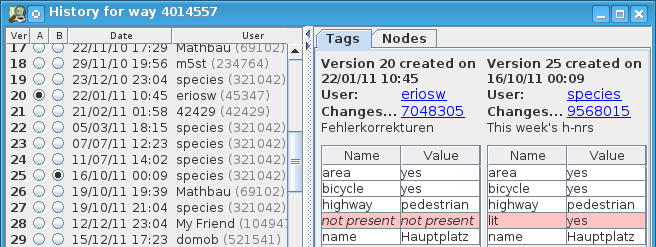
\includegraphics[width=8cm]{history.png}


\end{frame}

% Wie daraus Karten generieren:
% 1F Toolchain
% nF Beispiele:
% * irgendein Zoo Mapnik -OK
% * 3D
% * Tolle Kartenstile:
%     * OSM-Fr? -OK http://tile.openstreetmap.fr/ -OK
%     * stamen watercolor -OK http://maps.stamen.com/watercolor/ -OK
%     * pistemap /snow http://www.opensnowmap.org/ -OK
%     * bicycle map -OK http://cyclemap.org/ -OK
%     * OpenSeaMap -OK http://openseamap.org/ -OOK
%   show http://toolserver.org/~osm/locale/ru.html
    

\begin{frame}{Toolchain für Web-Karten}

Wie funktioniert die Kartenanzeige im Browser?
\pause

\begin{itemize}
  \item Javascript-Framework (zB Leaflet) lädt on Demand Kacheln (Tiles) vom Server
  \item Die Tiles werden von  Apache mit \emph{mod-tile} ausgeliefert
  \item mod-tile kontaktiert den Queue-Manager \emph{Tirex} für Renderjobs
  \item Tirex rendert mittels \emph{Mapnik}
  \begin{itemize}
    \item Mapnik-Stile sind XML, das mittels CartoCSS generiert wird
  \end{itemize}
  \item Mapnik bekommt die Daten von einer PostGIS-DB
  \item PostGIS-DB wird minütlich vom Hauptserver upgedated
\end{itemize}

Siehe Howto auf \url{http://switch2osm.org/}

\end{frame}


\begin{frame}{Freie Datendaten ermöglichen freie Kartenstile}

Der Standard-Kartenstil (Mapnik) ist auf \href{https://github.com/gravitystorm/openstreetmap-carto/}{Github} verfügbar
\begin{itemize}
  \item Kann für persönlichen Stil angepasst werden
  \item Er wird kollektiv weiterentwickelt, jeder kann mitmachen!
\end{itemize}

\begin{center}
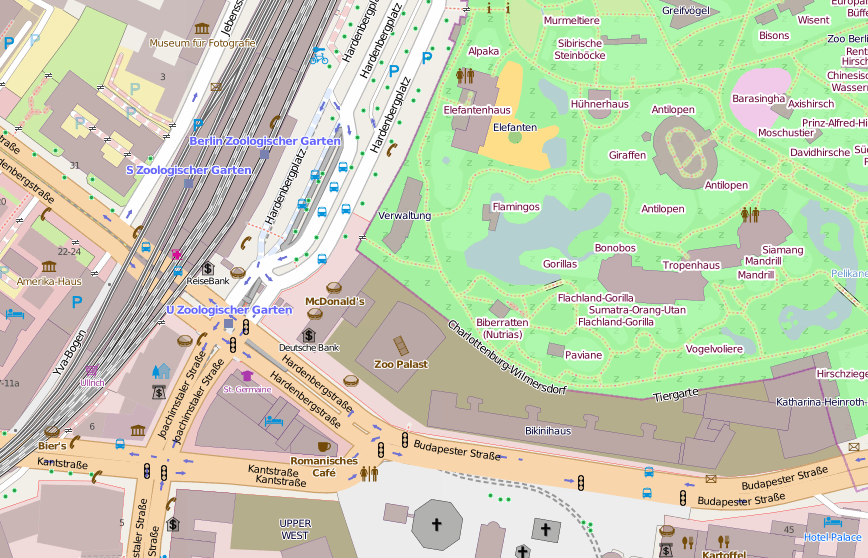
\includegraphics[width=7cm]{style-mapnik.png}
\end{center}

\vspace{-0.5cm}
weitere Stile: \url{http://wiki.osm.org/Featured\_tiles}

\end{frame}

\hypersetup{urlcolor=cyan}

\begin{frame}{Französischer Stil:\hfill\url{http://tile.openstreetmap.fr/}}
\begin{center}
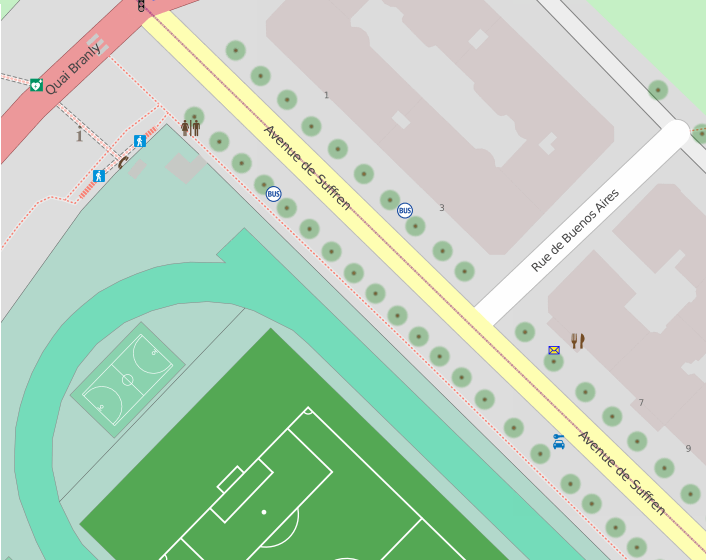
\includegraphics[height=7cm]{style-french.png}
\end{center}
\end{frame}

\begin{frame}{Stamen Watercolor:\hfill\href{http://maps.stamen.com/watercolor/}{http://maps.stamen.com/watercolor}}
\begin{center}
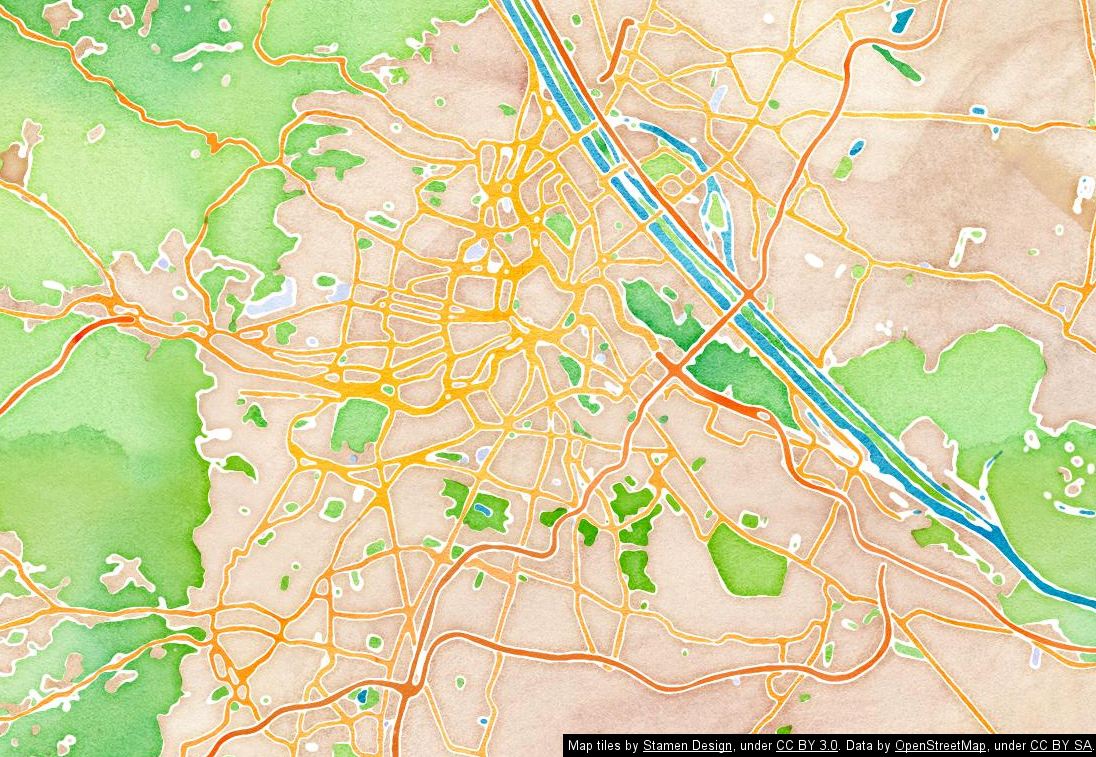
\includegraphics[height=7cm]{style-stamen.png}
\end{center}
\end{frame}
\hypersetup{urlcolor=blue}

% QA -TODO

\begin{frame}{Qualitätssicherung}
Ähnlich Wikipedia, jeder darf alles ändern!
  \begin{columns}[c]
    \begin{column}[T]{.35\textwidth}
      \vspace{1cm}
      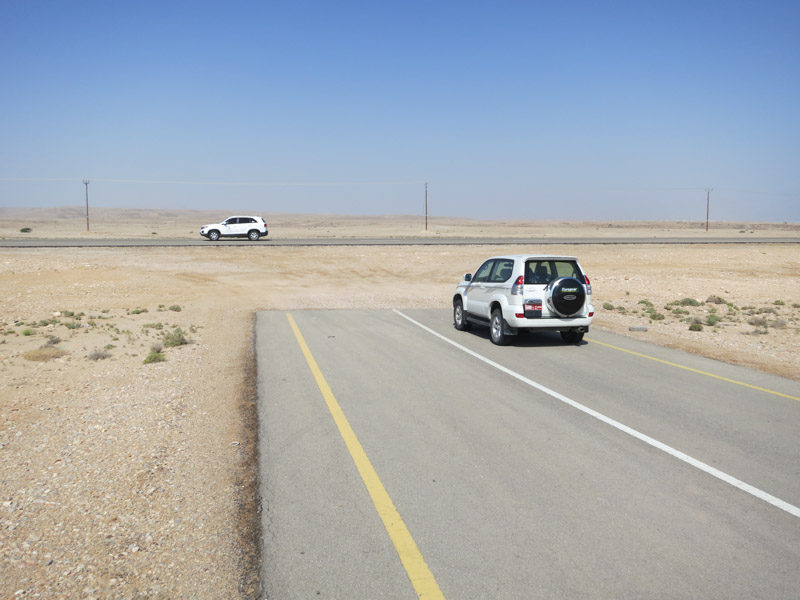
\includegraphics[width=4.5cm]{unconnected.jpg} \\
      {\TINY CC-BY \url{http://www.bodenseepeter.de}}
    \end{column}
    \pause
    \begin{column}[T]{.7\textwidth}
      \begin{itemize}
        \item Jedoch konfliktfreier als bei Wikipedia:
        \begin{itemize}
          \item Es gibt in OSM nur "`Ground Truth"'
          \item Eintrittsschwelle ist höher (keine Anonymous edits)
        \end{itemize}
        \item Erfahrene Mapper kontrollieren ihr Gebiet mittels RSS-Feed
        \pause
        \item Eingebautes Social Network: Jeder Mapper kann persönlich kontaktiert werden
        \begin{itemize}
          \item Diskussion über die Mailingliste
        \end{itemize}
        \pause
        \item Automatische Qualitätssicherungs-Tools
        \begin{itemize}
          \item \href{http://keepright.ipax.at/report\_map.php?zoom=14&lat=48.20808&lon=16.37221}{keepright.ipax.at}
        \end{itemize}
      \end{itemize}

    \end{column}
  \end{columns}

\end{frame}


\subsection{Datenmodell}

\begin{frame}{Datenmodell}
Wurde von Informatikern ohne Geo-Vorbelastung erstellt:
\begin{itemize}
  \item Punkte (Koordinaten), $\Rightarrow$ "`Node"' 
\includegraphics[width=0.5cm]{node.png}
  \begin{itemize}
    \item POIs
    \pause
    \item Teile von Wegen
  \end{itemize}
  \item Linienzüge sind eine Reihe von Nodes, $\Rightarrow$ "`Way"' 
\includegraphics[width=0.5cm]{way.png}
  \begin{itemize}
    \item Wege, Flüsse, Hecken etc.
    \item können geschlossen sein: Gebäude, Flächen
  \end{itemize}
  \pause
  \item Gruppierungen von Ways/Nodes $\Rightarrow$ "`Relations"' 
\includegraphics[width=0.5cm]{relation.png}
  \begin{itemize}
    \item Streckenrelationen, zB ÖPNV-Routen, Radrouten
    \item Multipolygone 
    \item Abbiegebeschränkungen (Way:von, Way:nach, Node:über)
    \item Meta-Relationen, zB für Verkehrsverbünde
  \end{itemize}
\end{itemize}

\end{frame}


\begin{frame}{Datenmodell: Tagging}

Jedes Element kann beliebige Anzahl Eigenschaften haben. 
Diese "`Tags"' genannten key=value Paare sind Freitext -- z.B.:
\begin{itemize}
  \item amenity = cafe 
\includegraphics[width=0.5cm]{cafe.png}
  \item highway = footway 
\includegraphics[width=1cm]{footway.png}
  \item building = yes  
\includegraphics[width=0.5cm]{building.png}
\end{itemize}

\pause
Dadurch ist man zu 100\% flexibel - und kann praktisch alles in die OSM eintragen, was einen Geobezug hat!

\begin{itemize}
  \item Straßen- und Wegenetz, Schiffahrtsrouten, Skipisten, \dots
  \item Flächen (Bewuchs, Landnutzung, Schutzzonen)
  \item POI-Eigenschaften wie Kontaktdaten, Öffnungszeiten, Rollstuhleignung, Nichtraucherschutz
\end{itemize}

Standards werden im Wiki festgelegt, siehe \href{http://wiki.openstreetmap.org/wiki/DE:How\_to\_map\_a}{wiki/DE:How\_to\_map\_a}

\end{frame}


\hypersetup{urlcolor=cyan}

\begin{frame}{Ski-Karte :\hfill\url{http://www.opensnowmap.org/}}
\begin{center}
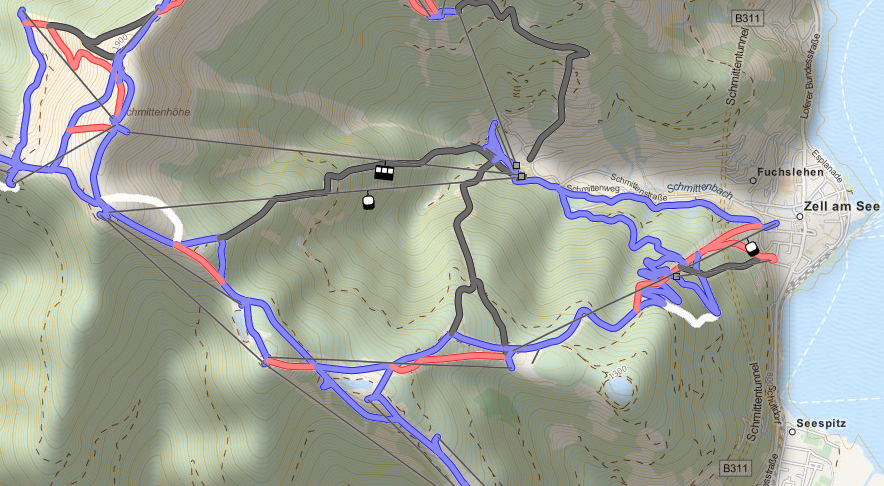
\includegraphics[height=6.1cm]{style-snow.png}
\end{center}
\end{frame}

\begin{frame}{See-Karte :\hfill\url{http://www.openseamap.org/}}
\begin{center}
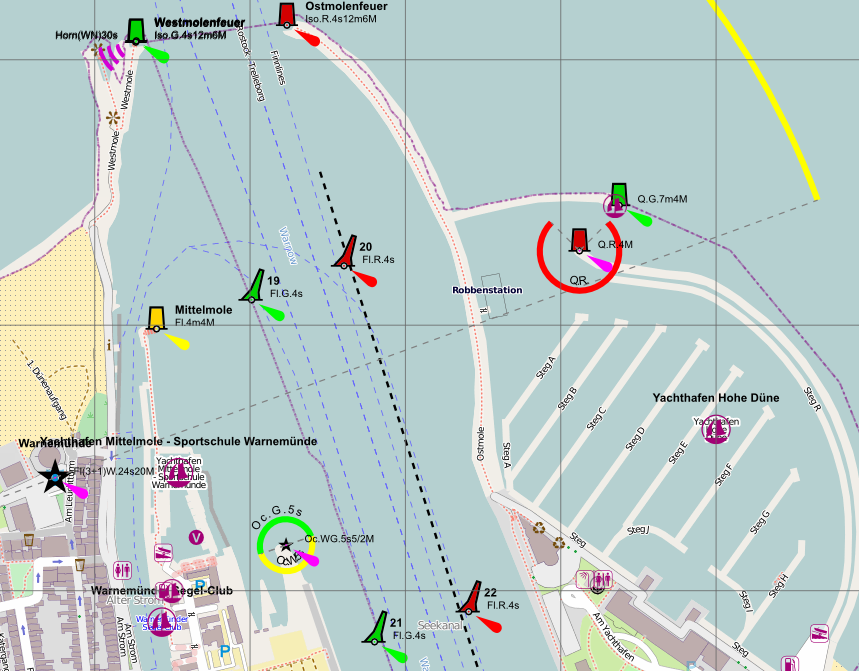
\includegraphics[height=7cm]{style-seamap.png}
\end{center}
\end{frame}

\begin{frame}{Fahrrad-Karte :\hfill\url{http://www.opencyclemap.org/}}
\begin{center}
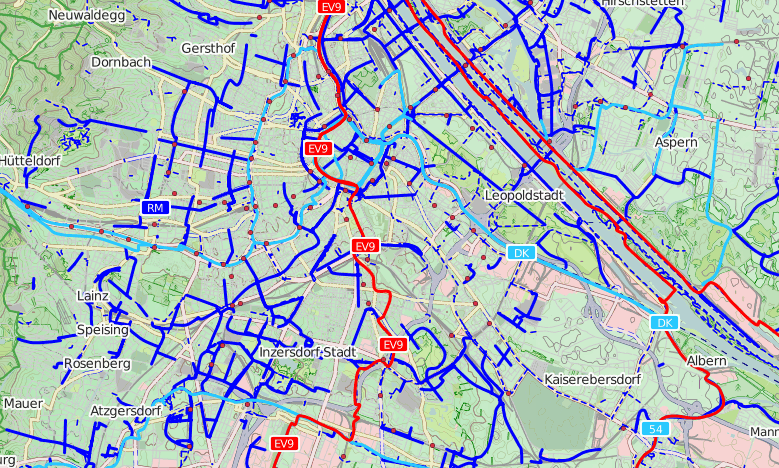
\includegraphics[height=6cm]{style-cycle.png}
\end{center}
\end{frame}

\begin{frame}{Datenmodell: Hintergrund}

Alle Standards möglichst offen:

\begin{itemize}
  \item Koordinaten sind in Dezimalgrad, WGS84.
  \begin{itemize}
  \item 3D-Information werden als Tags eingetragen, zb ele=435
\end{itemize}
  \item Genauigkeit 7 Stellen, entspricht 1\,cm am Äquator.
  \item Austausch-Dateiformate: XML, PBF (Binärkomprimierung für Geodaten von Google)
  \item 64bit-Kompatibel: Der 2-Milliardste Node wurde Anfang 2013 gesetzt.
\pause
  \item Zeichensatz UTF-8 $\Rightarrow$ Unterstützung aller Sprachen
\end{itemize}

\end{frame}


\hypersetup{urlcolor=blue}


\subsection{Lizenz}

\begin{frame}{Lizenz}

Die Daten stehen unter der Open Database Licence - Entspricht etwa Creative Commons - Attribution - Sharealike für Daten.
\begin{itemize}
  \item Jeder darf die Daten, auch kommerziell verwenden
  \item Quelle: "`OpenStreetMap and Contributors, ODbL"' muß angegeben werden.
\end{itemize}

 \begin{center}
 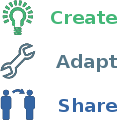
\includegraphics[width=1cm]{ODbL.png}
 \hspace{2cm}
 
\includegraphics[width=1.5cm]{cc-by-sa.pdf}
 \end{center}

\pause
Die Web-Karten auf \href{http://osm.org}{openstreetmap.org} sind CC-BY-SA.
\begin{itemize}
  \item Beachte Tile Usage Policy!
\end{itemize}


\end{frame}


% * OSM Nutzen: Rohdaten, Web-Dienste, Apps

% 3
% Rohdaten
%   link zu jedem punkt item
%   export als svg/osm.org
%   download von planet / shapefiles geofabrik
%   overpass (turbo)
% web-dienste
%   eigene kartenstile machbar
%      Tilemill
%      einige karten vorstellen 
%      Language-Independent
%   Geocoder
%   Routing
%   Notes-Feature
%   Web-Editor






\section{OpenStreetMap Nutzen}

\subsection{Rohdaten}

\begin{frame}{OSM-Daten Downloaden}

	Download von Rohdaten im osm-xml Format:
\begin{itemize}
	\item kleinen Bereich: \href{http://osm.org}{osm.org}, Export
	\item Full Planet: \href{http://planet.osm.org}{planet.osm.org}
	\item Länderextrakte: \href{http://download.geofabrik.de}{geofabrik.de}
	\item SQL-Like API: Overpass, Webinterface: \href{http://overpass-turbo.eu}{overpass-turbo.eu}
\end{itemize}
\pause
Export in andere Formate: 
\begin{itemize}
	\item Bilder (PNG, JPG, SVG, PDF): \href{http://osm.org}{osm.org}, "`Share"'-Icon rechts
	\item Shapefiles: \href{http://download.geofabrik.de}{geofabrik.de} (Limitierte Spalten)
	\item GeoJSON: \href{http://overpass-turbo.eu}{overpass-turbo.eu}
\end{itemize}

\end{frame}

\subsection{Dienste}

\begin{frame}{Dienste}
	Was bietet OpenStreetMap:
\begin{itemize}
	\item Geocoder: \href{http://nominatim.osm.org}{nominatim.osm.org}, Suche auf osm.org
		\pause
	\item Routing-Dienste für Auto, Fahrrad, Rollstuhl, \dots
		\pause
	\item Web-Karten zum Einbetten als HTML: \href{http://osm.org}{osm.org}, "`Share"'-Icon rechts
		\pause
	\item Links auf jedes einzelne OSM-Objekt; Marker
\end{itemize}

Wie das funktioniert $\Rightarrow$ Workshop Nachmittags

\end{frame}


\begin{frame}{Mobil Nutzen}
	Apps:
 
 \begin{itemize}
   \item  Android ( \textgreater 80) \url{http://wiki.osm.org/Android}
   \item  iPhone ( \textgreater 60 )  \url{http://wiki.osm.org/Apple\_iOS}
   \item  Blackberry ( 8 ) \url{http://wiki.osm.org/BlackBerry\_OS}
   \item  Windows Phone ( 13 ) \href{http://wiki.osm.org/Windows\_Phone}{wiki.osm.org/Windows\_Phone}
 \end{itemize}
 
 \begin{center}
 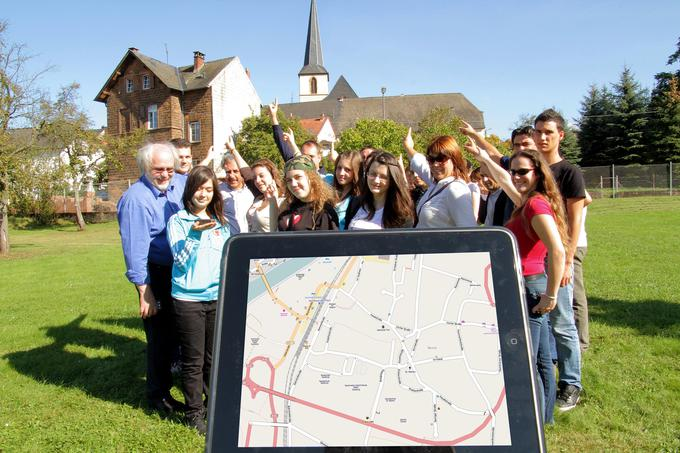
\includegraphics[width=5cm]{tablet.jpg}
 \end{center}

 Natürlich auch auf Navis, am OSM-freundlichsten sind Garmin: \href{http://wiki.osm.org/Garmin}{wiki.osm.org/Garmin}!

\end{frame}

  \subsection{ OpenStreetMap Verbessern}

\begin{frame}{OpenStreetMap Verbessern}

  Eine große Auswahl an Editoren steht fürs Web, Desktop- und Mobilnutzung zur Verfügung

  \begin{itemize}
    \item Web:
    \begin{itemize}
	    \item Hauptseite - Edit: iD (JavaScript)
      \item JOSM web-start
      \item oder auch einfach nur Fehler melden mit dem Note-feature auf \href{http://osm.org}{osm.org}!
	      \pause
    \end{itemize}
    \item Mobile (Auswahl): Alle siehe  \href{http://wiki.openstreetmap.org/wiki/Android\#OpenStreetMap\_editing\_features}{Android}, \href{http://wiki.openstreetmap.org/wiki/Apple\_iOS\#OpenStreetMap\_editing\_features}{iOS}:
    \begin{itemize}
      \item Vespucci: Ausgewachsener Editor
      \item osmaptuner: Existierende POIs ergänzen
      \item OsmTracker: GPS-Tracks, Audio, schnell POIs hinzufügen
    \end{itemize}
  \item Desktop
    \begin{itemize}
      \item \href{http://josm.openstreetmap.de}{JOSM}
      \item \href{http://merkaartor.be}{Merkaartor}
      \item ArcGIS (seit 10.1)
    \end{itemize}
  \end{itemize}

\end{frame}



\begin{frame}{Die Zukunft... 3D! }
  Neu! Jetzt auch in 3D! Beispielsweise auf \href{http://maps.osm2world.org/?zoom=17&lat=47.06156&lon=15.46983&layers=BF0FTFFF}{maps.osm2world.org}.

  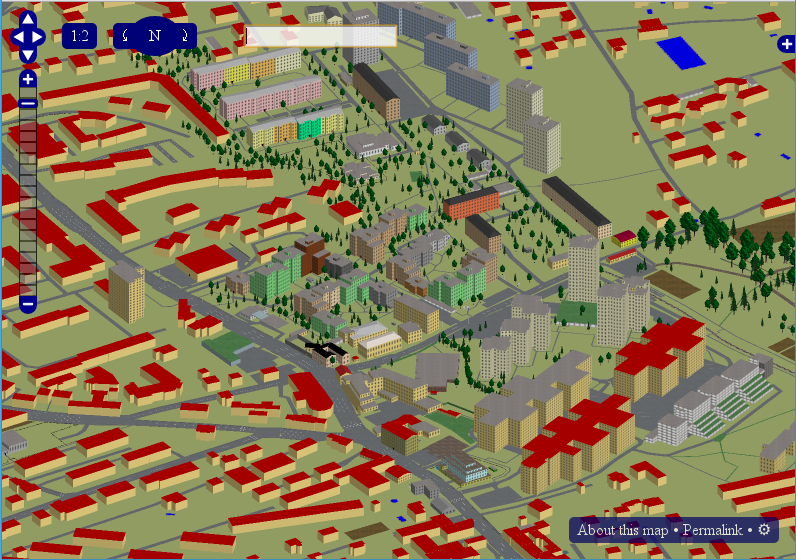
\includegraphics[width=0.9\textwidth]{3d.png}


\end{frame}

\begin{frame}{Hilfe}
Fragen? 
\begin{itemize}
  \item Dokumentation: \href{http://wiki.openstreetmap.org}{wiki.openstreetmap.org}
  \begin{itemize} 
    \item Mitmachen? \href{http://learnosm.org/}{learnosm.org}
  \end{itemize}
  \item Immer noch etwas unklar? $\Rightarrow$ Mailingliste \href{http://lists.openstreetmap.org/listinfo/talk-at}{talk-at}
  \item Weltweite \href{http://usergroups.openstreetmap.de/}{Stammtische}
  \begin{itemize}
    \item 1/Monat Wien
    \item 1/Monat Graz
    \item 1/Monat Innsbruck
  \end{itemize}

\end{itemize}

 \vspace*{-2.0cm}
\hfill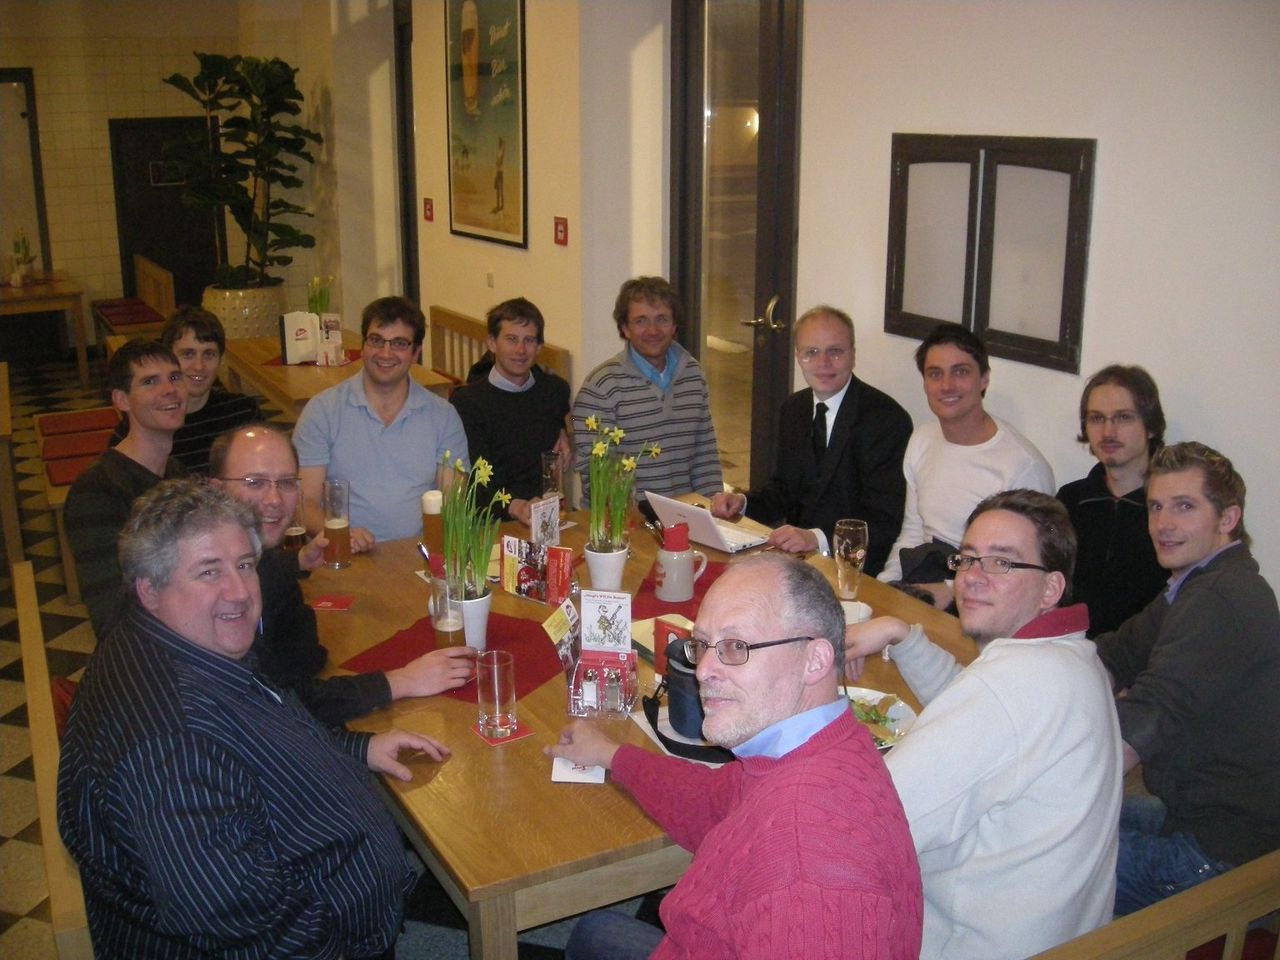
\includegraphics[width=5cm]{Salzburg_stammtisch.jpg}

\begin{itemize}
  \item Konferenz: \href{http://sotm-eu.org/}{State of the Map Europe}, 13.-15. Juni, Karlsruhe
\end{itemize}
\end{frame}

\section{Ende}

\begin{frame}{Vielen Dank für die Aufmerksamkeit!}

  Folien zu Themen zur Geovisualisierung am 9.4.2014, Graz
\vspace{1cm}

Erstellt mittels \LaTeX Beamer, Quelltext: \href{https://github.com/species/vortrag-osm-kfu-geovis}{Github}.
\vspace{1cm}

\href{mailto:michael.maier@student.tugraz.at}{Michael Maier}

Twitter: \href{https://twitter.com/osmgraz}{@osmgraz}
\vspace{1cm}

Folien unter: 
\includegraphics[width=1cm]{cc-by-sa.pdf}. 

Alle Daten ODbL, OpenStreetMap Contributors.

\end{frame}

\begin{frame}{Pause}

5 Minuten Pause \dots

\vspace{1.5cm}

Fragen? Jetzt!

\vspace{1.5cm}

Danach: OSM-Daten anzeigen mittels \href{http://overpass-turbo.eu}{overpass-turbo.eu}

\end{frame}

\begin{frame}{overpass-turbo.eu}

  Zur schnellen Darstelleung von Live-OSM-Daten

\begin{itemize}
        \item Use the Wizard! "`Pub in Graz"'
        \item Zoom to data (Lupe links)
        \item Try Load $\Rightarrow$ Examples $\Rightarrow$ MapCSS (Zoom in, Much data)
        \item Try Load $\Rightarrow$ Templates $\Rightarrow$ Key-Value mit Key aus OSM-Wiki
\end{itemize}

\pause
Aufgabe: Eine interessante, gestylte Map erstellen, und via "`Share"' den Link teilen

\end{frame}


\end{document}
